\documentclass[man, noapacite, 12pt]{apa2}

\makeatletter
\newenvironment{chapquote}[2][2em]
  {\setlength{\@tempdima}{#1}%
   \def\chapquote@author{#2}%
   \parshape 1 \@tempdima \dimexpr\textwidth-2\@tempdima\relax%
   \itshape}
  {\par\normalfont\hfill--\ \chapquote@author\hspace*{\@tempdima}\par\bigskip}
\makeatother

%\usepackage{pdfsync}
\usepackage{amsmath}
\usepackage{graphicx}
%\usepackage{topcapt}
%\usepackage{color}
%\usepackage{comment}
\usepackage{booktabs}
\usepackage{apacite2}
\usepackage{fullpage,rotating}
\usepackage{pslatex}
\usepackage{amssymb}
\usepackage{multirow}


\title{Linguistic structure emerges from cognitive mechanisms}
\author{Molly L. Lewis}
\affiliation{Department of Psychology, Stanford University\\ Conceptual Analysis of Dissertation Area\\ 6 October 2014}

\shorttitle{Linguistic structure emerges from cognitive mechanisms}
\rightheader{Linguistic structure emerges from cognitive mechanisms}
\acknowledgements{Advisor: Michael C. Frank\\ \noindent Additional Readers: Ellen Markman and Noah Goodman}

\abstract{People interact with people and, because of shared interest, try to coordinate their behavior. This behavior is governed by the competition of pragmatic pressures. These pressures lead to equilibria. These equilibria become conventionalized over time (Lewis). This convention becomes an additional pressure in the moment of interaction. Language as a paradigm case of these dynamics.}

\begin{document}
\maketitle

%%%%%%%%% INTRO %%%%%%%%% 
%\begin{chapquote}{Aristotle, \textit{Nic. Ethics II 6}}
%\noindent  Virtue, then, is a state of character concerned with choice, lying in a mean, i.e. the mean relative to us, this being determined by a rational principle, and by that principle by which the man of practical wisdom would determine it. Now it is a mean between two vices, that which depends on excess and that which depends on defect; and again it is a mean because the vices respectively fall short of or exceed what is right in both passions and actions, while virtue both finds and chooses that which is intermediate. Hence in respect of its substance and the definition which states its essence virtue is a mean, with regard to what is best and right an extreme.
%\end{chapquote}

\begin{chapquote}{G.K. Zipf, \textit{1949}}
\noindent  Human society can be viewed as a field which both influences the individual members of the group and is influenced by them. 
\end{chapquote}

\section{Introduction}
``Room for cream?'' asked the barista. ``Mm, yes -- just a bit" replied the customer. Mundane linguistic interactions such as this are the building blocks of daily experience. They are individuals making sounds to each other in an effort to coordinate their behavior in the physical world \cite{clark2006social}. These interactions are messy, variable, and highly unconstrained. Indeed it is this variability that gives language its vast expressive power \cite{hockett1960}. Yet, despite this appearance of irregularity, rich patterns in linguistic usage are revealed when we aggregate across instances of language use both within and across languages. At the level of syntax, for example, there is a strong bias in English to put subjects before verbs and, across languages, this pattern is attested more often than would be expected by chance alone  \cite{dryer2005order}. These types of probabilistic regularities exist at every level of linguistic structure --- from phonology, to semantics, syntax, and discourse --- and researchers from a variety of disciplines have taken as their project the goal of characterizing these regularities.

In this paper, I argue that we can gain  insight into the character of linguistic structure by considering the dynamics of language use. I will suggest the best way to do this is by framing language use as an instance of a broader phenomenon: social interaction \cite{clark1996using}. In particular, I will adopt the formal framework of social interaction proposed by Thomas Schelling, in which social interactions are viewed as acts of solving coordination problems.  To illustrate, consider the barista example above. In this example, the agents are the barista and the customer, and they must coordinate how  to fill the coffee mug. There are two outcomes --- full and almost full --- and the barista's desired outcome is determined by the preference of the customer. In this case, the barista and the customer rely on language to coordinate their behavior, but this coordination could have been achieved in other ways (e.g. the customer could have shook her head, pointed to the place inside the mug that she wanted the coffee filled to, etc.). Coordination of their behavior is achieved  by arriving at the mutually preferred outcome (the customer's mug is almost full).

A key tenet to the broader argument is that the act of using language is itself an act of solving a coordination problem \cite{clark1996using}. When a person speaks, there are many possible ways the utterance could be interpreted, and arriving at the intended interpretation is an act of coordination. For example, in the case of the customer's interaction with the barista, there are many possible interpretations of the phrase, ``Room for cream?." The barista could mean ``Would you like to add cream to your coffee? If so, I will facilitate that by not filling your mug full with coffee." Or, ``We have so much extra inventory of cream! Do you have room in your bag to take some?" Or, ``Do you like the band `Room for cream'?". Or, if the speaker is speaking another language, a totally unrelated meaning. The point is that the speaker's intended meaning is underspecified from the language alone and the interlocutors must work collaboratively to arrive at a shared understanding. Following \citeA{lewis1969convention}, I will suggest that we can gain insight into the dynamics of linguistic coordination problems such as this by using Schelling's formal framework.  This perspective on language use will ultimately provide a helpful framework for understanding the relationship between language use and language structure.

It is worth reflecting on the historical relationship between these two aspects of language. In this study of language, there has been a tension between whether the data to be explained should be instances of language use or structural regularities that emerge across speakers. Theoriests take different perspectives on the ontological status of these structural regularities -- Chomsky exists in the head, saussure, a social fact. But, they agree that the regularities across are what is important.In particular, they have been presented in opposition. 
% A historical asside -- a tension between studying messy in the moment pragmatics (Saussure, langue Parole, Labov). Canton paper
The goal of this paper is to suggest that, not only are these two aspects of language deeply related to each other, the key to understanding linguistic structure may lie in understanding linguistic use.

In Part I, I will outline the linguistic coordination problem as a paradigmatic case of the social coordination problem. I will suggest that coordination problems are solved through the dynamics of two opposing two forces --- the goals of the one's self and the goal of the other. Following Lewis, I suggest that these opposing forces are resolved by finding an equilibrium point. I will then argue that the equilibria that are reached in language use are reflected in the structure of language, and survey a variety of phenomena in linguistic structure that show this pattern.

In Part II, I will consider the mechanism that might cause linguistic structure to reflect the equilibria reached in linguistic use. Lewis argued that once individuals succeed in solving a coordination problem, there is a tendency to stick with that solution (even though other, equally good solutions exist). This solution is called a convention. I will argue that the key to understanding the link between regularities in linguistic usage and linguistic structure is the process of children's acquisition of these conventions. I will consider how the dynamics of language acquisition might lead to language change. Finally, I will consider the complementary role of conventions and cognitive forces in solving language coordination problems, and the  empirical challenge associated with disentangling the two.

%%%%%%%%% PART I %%%%%%%%% 
\section{Part I: Linguistic structure reflects pragmatic equilibria}

Where does linguistic structure come from? \citeA[2010]{christiansen2008} propose a compelling theory. They argue that  multiple cognitive constraints dynamically influence language evolution. They suggest four constraints: the representational format of thought, properties of the percepto-motor system, learning and processing constraints, and constraints that result from reasoning about others intentions ({\it pragmatic} constraints). Their argument is that these  cognitive constraints  influence  language at the moment of use, but over time, these biases become instantiated in the structure of language. Although each of these constraints likely plays an important role in the evolution of language, the present paper focuses on the independent contribution of pragmatic constraints. The claim is that pragmatic constraints that play out at the moment of language use become fossilized in the structure of language over time. To develop this claim, we begin by modeling language use as a type of social coordination. We then turn to an analysis of language use as a social coordination problem. Finally, we consider cases where there are similarities in phenomena between language use and language structure.

\subsection{Social interaction as a coordination problem}
Many theorists of language \cite{zipf1936, lewis1969convention, grice1975logic, clark1996using} have observed that language is an instance of a much broader class of behavioral phenomena --- social coordination. For each, language use is a case of multiple agents making interdependent  rational choices.\footnote{In outlining his seminal theory of pragmatics, Grice  writes: ``As one of my avowed aims is to see talking as a special case or variety of purposive, indeed rational, behaviour, it may be worth noting that the specific expectations of presumptions connected with at least some of the foregoing maxims have their analogues in the sphere of transactions that are not talk exchanges" \cite[pg. 47]{grice1975logic}.} By adopting work from game theory,  \citeA{lewis1969convention} formalized the notion of language as a coordination problem. He defines a  {\it coordination problem} as follows: \begin{quote} Two or more agents must each choose one of several alternative actions. Often all the agents have the same set of alternative actions, but that is not necessary. The outcomes the agents want to produce or prevent are determined jointly by the actions of all the agents (p. 8).
\end{quote} 
The key feature of these problems is that some combinations of the agents' choices are better than others: there are a set of equilibria of joint choices in which no agent would have a larger payoff had the agent alone changed her choice.

This broad framing can describe the dynamics of many social interactions. Take the above case of the barista and the customer, for example. We can model this interaction using a payoff matrix (Table 1). In the matrix, we represent the customer's payoff along the rows and the barista's payoff along the columns. There are two possible choices for  level of coffee in the cup---  full and  almost full --- and so each agent gets two rows or columns. 
\begin{table}[t]
\begin{center}
\begin{tabular}{l p{3cm} l p{3cm} l p{3cm} r}
 &  & \multicolumn{2}{c}{customer} \\ \cline{2-4} 
\multicolumn{1}{l|}{} & \multicolumn{1}{l|}{} & \multicolumn{1}{l|}{full} & \multicolumn{1}{l|}{almost full} \\ \cline{2-4} 
\multicolumn{1}{c|}{\multirow{2}{*}{barista}} & \multicolumn{1}{l|}{full} & \multicolumn{1}{l|}{0,0} & \multicolumn{1}{l|}{0,0} \\ \cline{2-4} 
\multicolumn{1}{c|}{} & \multicolumn{1}{l|}{almost full} & \multicolumn{1}{l|}{0,0} & \multicolumn{1}{l|}{1,1} \\ \cline{2-4} 
\end{tabular}
\caption{A payoff matrix of a context of a simple interaction --- a barista trying to determine how full to fill a customers' cup. Given the customer's preference for cream, there lies an equilibrium point at `almost full' for both barista and customer. To arrive at this equilibrium point, the two must coordinate.}
\end{center}
\end{table}
The agents relative payoffs are indicated in the cells, with the barista's on the left, and the customer's on the right. This happens to be a very simple equilibria --- there is one, and only one, possible set of actions in which is an equilibrium. The customer prefers almost full and the barista fills the cup to almost full. The problem is that the barista does not know a priori where this equilibrium lies, i.e. that the customer's pay off for almost full is 1, relative to 0 for full. To solve this coordination problem, the customer and barista make use of language.

More complicated coordination problems arise when there are multiple possible equilibria. Consider a weekend trip in which food and alcohol must be brought. To distribute the burden, half of the vacationers will bring food and the other half alcohol. In this case, the pay off matrix might look something like Table 2. Neither group --- Group A or B --- has a strong preference about which of the two commodities each brings. However, what is important is that one group brings food and the other alcohol (no one will be happy on a weekend trip with only food or only alcohol). There are thus two equilibria, one  at each set of choices where the two groups bring different things. By chance, the vacationers are equally likely to end up in a non-equilibrium as they are an equilibria. They must  therefore coordinate, via language or some other means, to ensure that they end up at an equilibrium.

\begin{table}[t]
\begin{center}
\begin{tabular}{l p{3cm} l p{3cm} l p{3cm} l}
 &  & \multicolumn{2}{c}{Group A} \\ \cline{2-4} 
\multicolumn{1}{l|}{} & \multicolumn{1}{l|}{} & \multicolumn{1}{l|}{food} & \multicolumn{1}{l|}{alcohol} \\ \cline{2-4} 
\multicolumn{1}{c|}{\multirow{2}{*}{Group B}} & \multicolumn{1}{l|}{food} & \multicolumn{1}{l|}{0,0} & \multicolumn{1}{l|}{1,1} \\ \cline{2-4} 
\multicolumn{1}{c|}{} & \multicolumn{1}{l|}{alcohol} & \multicolumn{1}{l|}{1,1} & \multicolumn{1}{l|}{0,0} \\ \cline{2-4} 
\end{tabular}
\caption{A payoff matrix for a social interaction in which there are two equilibria. Neither group cares who brings what commodity on the vacation; they only care that they bring different things. }
\end{center}
\end{table}

What are the psychological forces that support these coordination games? Zipf's theory of human behavior (1949) provides  insight. He argued that all human behavior could be accounted for by a single principle: people are motivated to minimize their effort ({\it The Principle of Least Effort}).  According this this principle, in a context in which individuals need to exert some physical effort, say in walking to a park --- they should be motivated to find the solution that minimizes how much effort required. Critically, Zipf argued this simple principle had explanatory power at the level of social groups. He suggested that this principle governs the behaviors of individuals, but with interaction, this principle leads to an equilibrium in behavior at the level of the group.

This simple theory of behavior provides a parsimonious account of a wide range of social phenomena. A particularly clear example is the organization of people into social  groups in physical space \cite{zipf1949human}.\footnote{A second, well-studied example is economics. At the the level of the individual, the consumer tries to minimize something of value, but in this case the valued commodity is money, rather than energy (though these are arguably related in important ways). This is the study of microeconomics. With interaction among consumers, this single force leads to regularities at the level of the social group, or the economy--- the study of macroeconomics.} Zipf assumes that every individual in a society is both a consumer and producer of goods. Governed by the Principle of Least Effort, the individual should minimize effort in terms of movement across land, by consuming (i.e.\ living) and producing (i.e.\ working) at the same location. However, as the number of raw goods increases this becomes increasingly difficult because the consumer cannot not live at the doorstop of every finishing plant. This creates a conflict. On the one hand there is a force to diversify, so that the population lives at the doorstep of the production line. This creates a force for many separated communities in space, each producing a single good, but with little trade between other communities. On the other hand, there is force to unify so that it is easier to trade final goods. The result is an equilibrium where people live in many different urban centers across the land. This general theory is reflected in more modern theories of urban spatial layouts \cite{mills1967aggregative, brueckner1987structure}.

Importantly, Zipf's principle does not provide a description of how individuals come to solve pure coordination problems like the vacationer example above. In that case, it is not clear how two individuals with the exact same payoff structure would arrive at the same, otherwise arbitrary solution. To address this issue, we need the idea of {\it convention} which will return to in Part II. However, Zipf's principle does provide insight into how a single psychological force, shared by all individuals, can lead to biases for different alternatives (e.g., a preference for the shortest path to a location). When individuals with these same biases interact with each other, we see the emergence of an equilibrium. 

\subsection{Language use as a coordination problem}
The coordination  framework can be straight-forwardly applied to language use \cite{lewis1969convention}. Language use is a paradigmatic case of a coordination problem because it is a tool that is universal in a community, easy to use, and capable of expressing complex ideas. In the case of language, the core of the coordination problem lies in the resolution of reference. Broadly, resolving reference requires interpreting a meaning from some utterance. At the level of individual lexical items, this is a difficult problem because the relationship between linguistic form and meaning is arbitrary \cite{saussure, hockett1960}. That is, knowing the form of a word does not give a language user any insight into the meaning of that word. Consequently, there is no inherent mapping between form and meaning and speakers must coordinate their behavior. 

\begin{table}[t]
\begin{center}
\begin{tabular}{l p{3cm} l p{3cm} l p{3cm} l}
 &  & \multicolumn{2}{c}{Speaker 1} \\ \cline{2-4} 
\multicolumn{1}{l|}{} & \multicolumn{1}{l|}{} & \multicolumn{1}{l|}{``fep"} & \multicolumn{1}{l|}{``dax"} \\ \cline{2-4} 
\multicolumn{1}{c|}{\multirow{2}{*}{Speaker 2}} & \multicolumn{1}{l|}{Object A} & \multicolumn{1}{l|}{0,0} & \multicolumn{1}{l|}{1,1} \\ \cline{2-4} 
\multicolumn{1}{c|}{} & \multicolumn{1}{l|}{Object B} & \multicolumn{1}{l|}{1,1} & \multicolumn{1}{l|}{0,0} \\ \cline{2-4} 
\end{tabular}
\caption{A payoff matrix of the mapping problem. Given two words and two referents, the mappings are arbitrary. The only constraint is that no word should map to more than one object, and no object should map to more than one word. Thus, as in the vacationer example, speakers must coordinate.}
\end{center}
\end{table}

The arbitrariness of linguistic form leads to a formal equivalence between the problem of reference and the problems of coordination described above.  To understand this similarity, consider  a case where  there are two novel words, ``dax" and ``fep," and two novel objects, Object A and Object B. Given this information alone, the listener has no a priori insight into which object each word refers to. This is a problem because the two interlocutors must somehow arrive at the same mappings between words and referents in order to communicate (a system in which you call Object A ``fep" and I call it ``dax" is a terrible communication system). The interlocutors must therefore coordinate. 

The payoff structure for this problem is identical to the vacationer example above (Table 3). Because language is arbitrary, neither speaker cares whether you call Object A ``fep" or ``dax;" they only care that their mappings are the same.  These general dynamics are true not only of individual lexical items, but of all cases of reference. Consider again our example of the barista and the customer. In interpreting the phrase, ``Room for cream?," the individual lexical items are relatively unambiguous --- presumably both know what ``room" and ``cream" mean. But, the intended meaning of the entire phrase is underspecified, and so the interlocutors must work together to resolve meaning.

In this framework, we can think of {\it pragmatics} as the study of the psychological processes that lead to an equilibrium in these referential coordination problems. Pragmatics, then, is just a specific case of the dynamics described by \cite{zipf1949human}. In the case of language, Zipf's insight was that speech could be thought of as its own economy, similar to any other social system. Speech has a physical cost and could be used as tool. He suggested the speaker and the listener were both governed by the Principle of Least Effort and this lead to an equilibrium. In the case of the speaker, effort could be minimized if there existed a single word {\it w} that could be used to refer to the set of all concepts {\it C}. In the case of the listener, effort would be minimized (in terms of understanding) if there existed a unique word for each  unique concept {\it c}. The dynamics of the interaction of these two opposing forces is pragmatics. 
%synthesis of two antitheses (horn, 22)
Many theorists have tried to account for pragmatic regularities in behavior, most notably \citeA{grice1975logic}. However, \citeA{horn1984} presents a particularly parsimonious theory that closely aligns with Zipf's more general formulation. He posited two principles that describe the manifestation of Zipf's Principle of Least Effort for the speaker and the hearer each. 
\begin{quote} \textsc{speaker}: Say no more than you must. ({\it Principle of Necessity}) \end{quote}
\begin{quote} \textsc{hearer}: Say as much as you can. ({\it Principle of Sufficiency})\footnote{Horn refers to these as the {\it R} and {\it Q} principles, respectively. I've opted  for less opaque terminology.} \end{quote}
These principles are quite straight forward. As a speaker with a necessary meaning to contribute, you want to say a little as possible, while still conveying the intended meaning. In contrast, as a listener, you want the speaker to say as much as possible to minimize your effort at arriving at the correct interpretation. That is you want the speaker to use sufficient language. In the limit, each strategy on its own does not result in a successful communication system. This is because the speaker's and the hearer's goal are fundamentally linked: While in the short term, in might be less effort for the speaker to utter a single sound, ``blah," to convey her meaning, this will lead to confusion on the part of the hearer, which the speaker will then have to clarify with additional language. The speaker and hearer must therefore resolve their two opposing forces  in what Horn called a ``division of pragmatic labor"  in order to arrive at an equilibrium point \cite[p. 22]{horn1984}.\footnote{Note that there is a super maxim that is also operating here: the cooperative principle \cite{horn1984, grice1975logic}. The cooperative principle is essentially the idea that the interlocutors realize that utterances are the result of an equilibrium from the dynamics these two forces. Put another way, it is a statement that the interlocutors realize that they are playing a coordination game.}

\begin{figure}
\begin{center} 
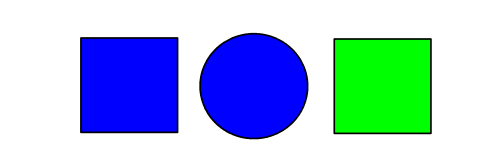
\includegraphics[width=3in]{figs/frank2012.png}
\caption{\label{fig:frank2012}  Example stimuli from Frank and Goodman (2012). In this case, the intended referent is the middle shape. Both speaker and hearer agree that utterance ``circle" is  an equilibrium point, as compared to ``blue," even though both terms equally describe the intended referent in truth-functional terms.}
\end{center} 
\end{figure}

While these principles are simple, the dynamics they give rise to are complex. \citeA{frank2012predicting} present a formal model that captures these dynamics in a simple reference game. In their game, there are three possible referents and each referent has two relevant features (Fig.\ 1). Given the constraint that a speaker can only utter a single word, there are always two possible words the speaker could utter. For example, if the  intended referent is a blue circle, a speaker could use either the word ``blue" or ``circle" to refer to the object. Critically, both words are equally true of the referent from the perspective of truth functional semantics. The phenomenon that this model captures is that the speakers use different words to refer to an object --- and that listeners expect them to --- depending on the context in which the word is uttered. In particular, speakers  tend to choose a word that most uniquely identifies the intended referent, given the referential context. In other words, they select the word that is most informative. For example, in the example trial pictured in Figure 1, speakers tend to use the word ``circle" instead of ``blue'' to identify the middle referent.  Frank and Goodman use a Bayesian framework to formalize this notion of informativity, and their model closely captures the behavioral data in this reference game. This suggests that the behavior of both interlocutors is guided by a tacit understanding of informativity in the referential context. 

This notion of informativity falls directly out of Horn's principles. In this reference game, speakers are constrained by the length of the utterance they can use (one word), but the choice of words is free. From the listener's perspective, the utterance must be sufficient and so uttering ``blue" would be insufficient in the above context because it is ambiguous, and there is a better alternative. From the speaker's perspective, the utterance must be necessary, but should not be too verbose. This force is enforced by structure of the task --- the speaker must contribute something to participate in the task, and the utterance cannot be overly verbose given the single word constraint. Maximal informativity --- a sufficient contribution, given the context --- is thus the equilibrium between these two forces.

\subsection{Pragmatic equilibria reflected in the structure of language}

Simple reference games like that of \citeA{frank2012predicting} are one example of the kind of equilibria that emerges from the interaction of Horn's principles, but there are many others. In the present section, we consider how these  pragmatic equilibria points in language use are reflected in the structure of language. We will consider this relationship for three different kinds of linguistic structure: semantics, words, and syntax.

\subsubsection{Semantics}
Semantics concerns the context-independent meaning associated with a word. The size of the semantic space denoted by particular word is the result of an equilibrium point between Horn's speaker and hearer principles.  From the hearer's perspective, Horn argues there is a pressure from  to narrow semantic space \cite{horn1984}. This reflects the idea that the hearer's optimal language is one in which every possible meaning receives it's own word. One example of this is the word ``rectangle." This word refers to a quadrilateral with four right angles. A special case of a ``rectangle"  is a case where the four sides are equal in length, which has its own special name, ``square." Consequently, the term ``rectangle" has been narrowed to mean a quadrilateral with four right angles, where the four sides are {\it not} equal.\footnote{Horn also points out that there are cases of narrowing that are speaker-based, as in ``drink" for ``alcoholic drink."} From the speaker's perspective, there is a pressure for semantic broadening. This is because the speaker's ideal language is one in which a single word can refer to a wide range of meanings. An example of this is the broadening of brand names to refer to a kind of product. For example, ``kleenex" is a name of a product name for facial tissues, but has taken on the meaning of facial tissues more generally.

The opposition of these two semantic forces predicts an equilibrium in the organization of semantic space that satisfies the pressures of both speaker and hearer. A body of empirical work has tested this prediction by examining the organization of particular semantic domains cross-linguistically \cite{regierword}. Languages show a large degree of similarity in how they partition semantic space for a particular domain, which is likely due to universal cognitive constraints. But, they also show a large degree of variability and these different systems can be shown to all approximate an equilibrium point between speaker and hearer pressures. 

 \citeA{kemp2012kinship} demonstrate this systematicity in the semantic domain of kinship. For each language, they developed a metric of the degree to which  Horn's speaker and hearer pressures (in their terminology: communicative cost and complexity, respectively) are satisfied. A language that better satisfies the hearer's pressure is one that is more complex, as measured by the length of the description of the system in their representational language. A language that better satisfies the speaker's pressure is one that requires less language to describe the intended referent. To understand this, consider the word ``grandmother" in English: this word is ambiguous in English because it could refer to either the maternal or paternal mother, and so referring to one in particular is more costly in English than in a language that encodes this distinction lexically. They find that the set of attested languages is a subset of the range of possible languages, and this subset are all partitions that are near the optimal tradeoff between speaker and hearer pressures (Fig.\ 2). This type of analysis has also been done for the domains of color \cite{regier2007color}, light \cite{baddeley2009relationship}, and numerosity \cite{xu4numeral}.
 
 \begin{figure}
\begin{center} 
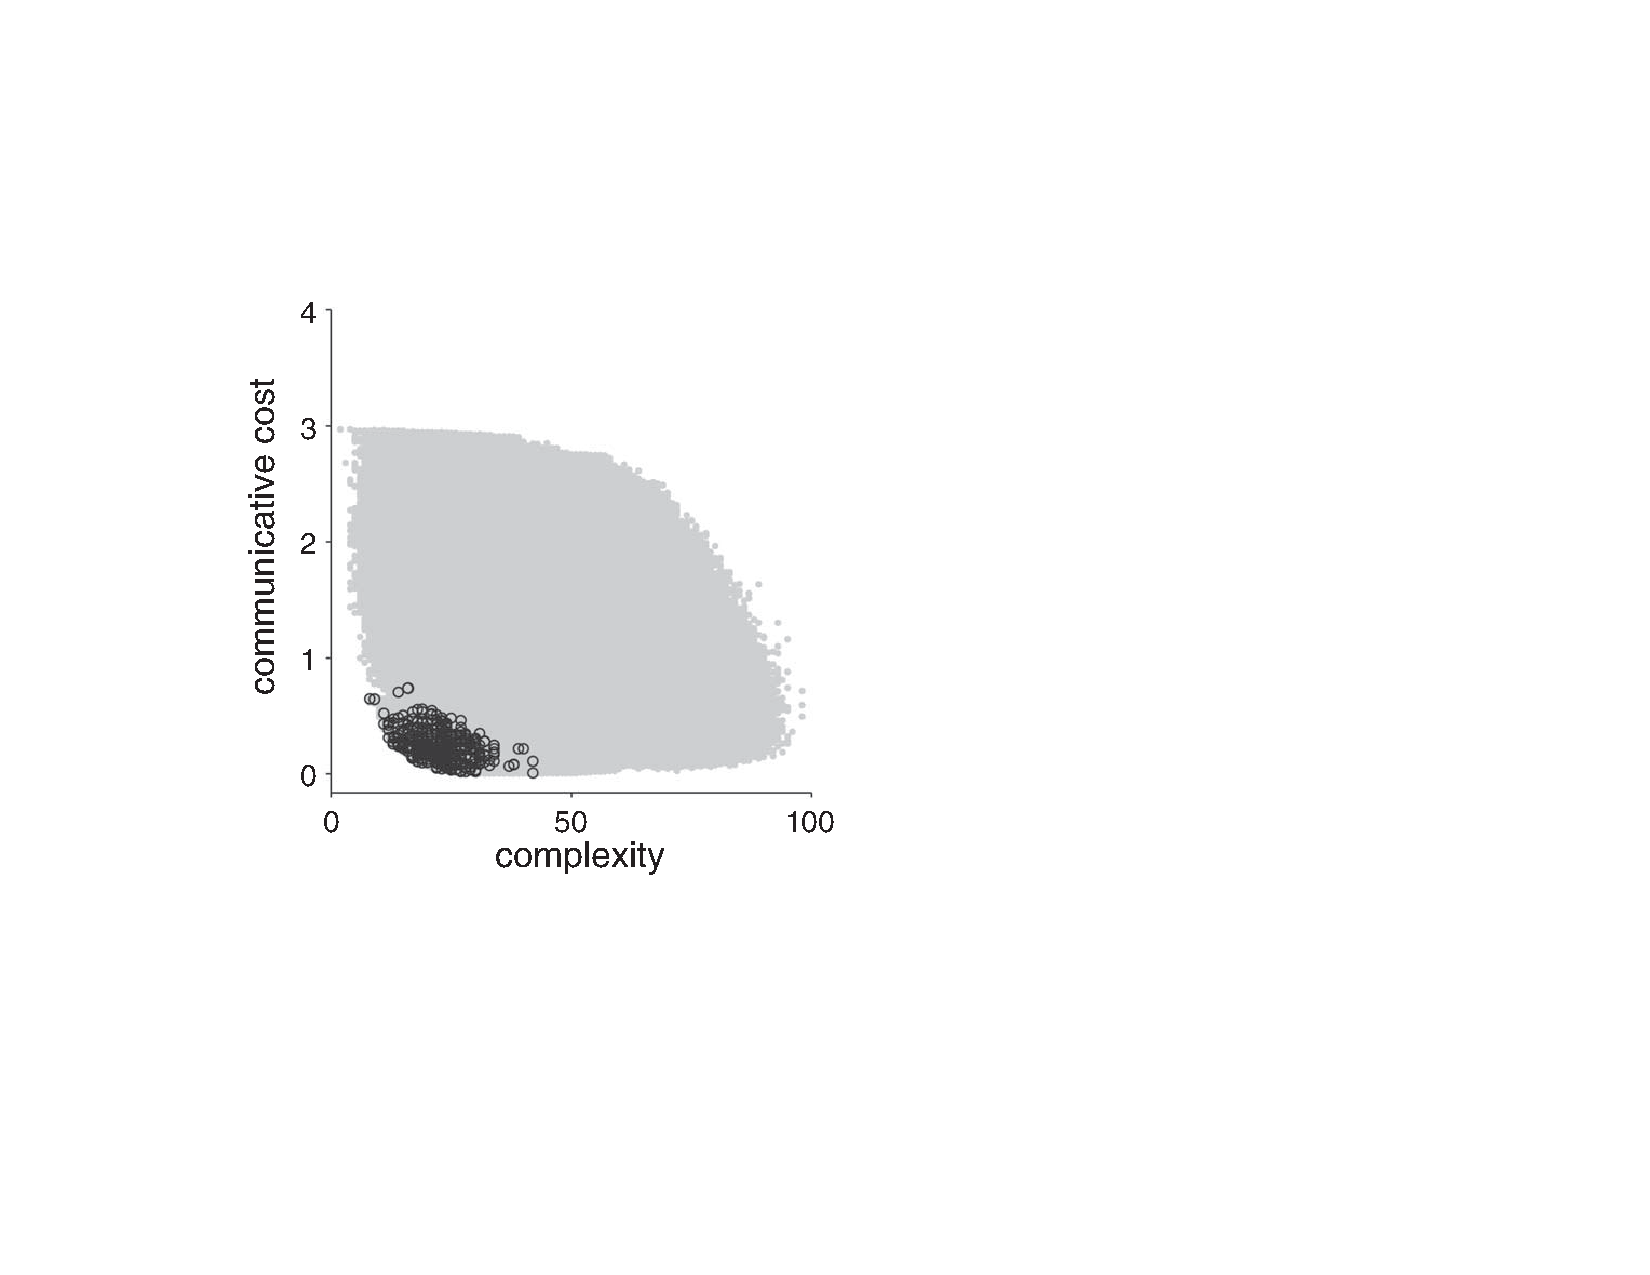
\includegraphics[width=2in]{figs/kemp2012.pdf}
\caption{\label{fig:frank2012} Plot  from Kemp and Regier (2012). Languages organize the semantic space of kinship in a way that optimizes both speaker and hearer pressures. The notion of {\it communicative cost} maps onto Horn's speaker principle and the notion of {\it complexity} maps onto Horn's hearer principle. Gray circles represent possible systems and black circles represented actually attested languages. The key observation is that all of the attested languages are clustered around the bottom left corner that corresponds to an equilibrium between speaker and hearer pressures.} 
\end{center} 
\end{figure}

A second phenomenon that is predicted by these forces is the presence of lexical ambiguity. That is, cases in which there are multiple meanings associated with a word, from a context-independent perspective. Language is rampant with examples of this. For example, the word ``bat" could mean either the instrument used in baseball or the flying mammal. This type of ambiguity in context-independent meaning is tolerated because the meaning is usually easily disambiguated by context. When the word ``bat" is uttered while watching a baseball game,  the mammal usage of the word is very unlikely. We can view the presence of this ambiguity as an equilibrium in Horn's speaker and hearer principles. If the meaning of a word can be disambiguated by the referential context, then it would violate the speaker's principle to have an overly-specific term for a meaning. 

Indeed, recent work by \citeA{piantadosi2011b} reveals systematicity in the presence of lexical ambiguity in language. They argue that ambiguity results from a speaker based pressure to broaden the meaning of a word to include multiple possible meanings. In particular, they suggest that this pressure should lead to a systematic relationship between the presence of ambiguity and the cost of a word. According to their argument, costly words (in terms of length, frequency, or any metric of cost) that are easily understood by context violate the speaker's principle to say no more than you must. Consequently, there should be a pressure for these meanings to get mapped on to a different, less costly word. This word may happen to already have a meaning associated with it, and so the result  is multiple meanings being mapped to a single word. For example, in the case of the word ``bat," a speaker could instead say ``baseball bat," but because this referent is easily disambiguated in context from the mammalian meaning,  Horn's speaker principles leads to a pressure to use the shorter form.\footnote{There are also cases of temporary ambiguity in the meanings of syntactic structures. For example, in a sentence that begins ``The coach knew you..." it is unclear whether ``you" is a direct object or the subject of a relative clause. Speakers can avoid this ambiguity by inserting a ``that," but this is optional. Work by \citeA{ferreira2000effect} suggests that speakers often do not avoid this ambiguity, presumably because the intended meaning can easily be recovered from context.} This leads to a testable prediction that shorter words should tend to be more ambiguous.  Through corpus analyses, \citeA{piantadosi2011b} find this precise  relationship between cost and ambiguity. They find a linear relationship between word length and ambiguity across English, Dutch and German: Shorter words are more likely to have multiple meanings. 

An additional case of this lexical ambiguity is found in words that have very little context-independent meaning, known as indexicals or deictics \cite{frawley2003international}. These words get their meaning from the particular referential context of the utterance, and are therefore highly ambiguous from a context-independent perspective. There are many types of indexicals that are present to varying degrees across languages. An example of temporal indexical form is ``tomorrow." The context-independent meaning of this word is something like ``the day after the day this word is being uttered in.'' Critically, abstracted from any context, this word has little meaning; it is impossible to interpret without having knowledge about the day the word was uttered. This phenomenon is also present in person pronouns (e.g.\ ``you" and ``I") and spatial forms, like ``here" and ``there."  As for lexical ambiguity, this type of ambiguity is a predicted equilibrium point from Horn's principles: If the hearer can recover the intended referent from context, the speaker would be saying more than is necessary by using an overly-specific referential term. Language structure reflects this pressure through lexicalized ambiguity in the form of indexicals.

\begin{figure}
\begin{center} 
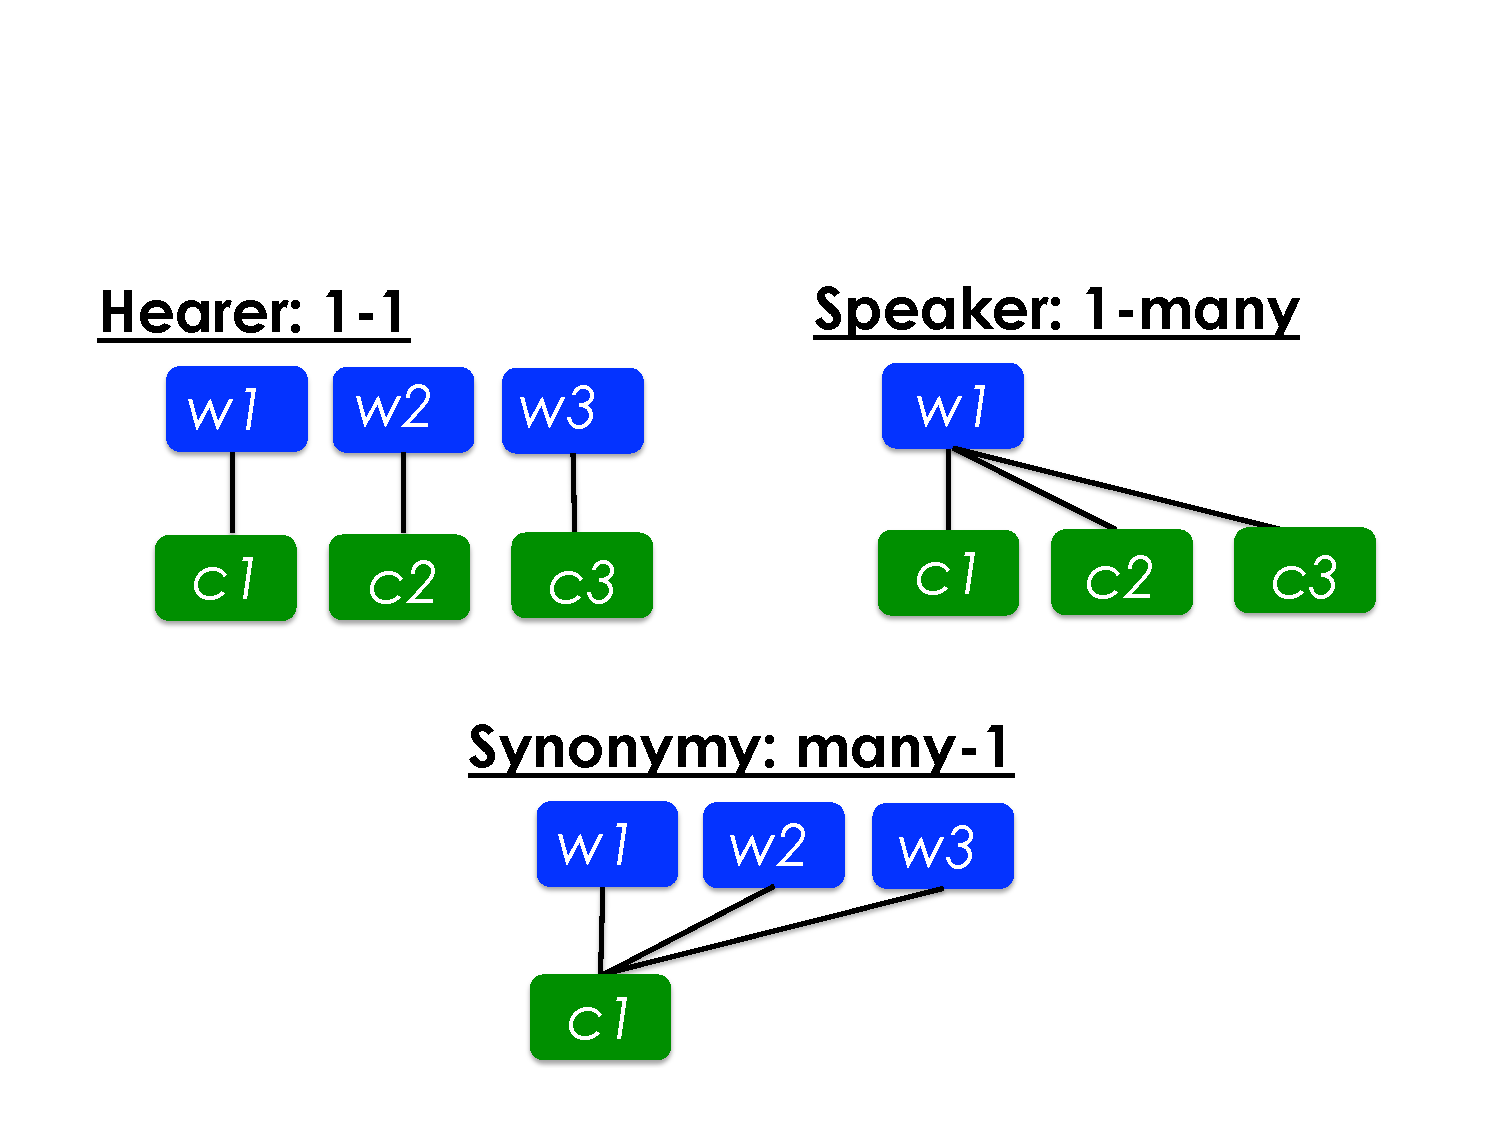
\includegraphics[width=3in]{figs/onetoone.pdf}
\caption{\label{fig:frank2012} Three possible structures on the organization of lexicon. According to Horn's principles, the hearer's optimal language is one in which there is a one-to-one mapping between words and concepts. The speaker's optimal language is one in which there is one word that maps to many concepts. Synonymy, or a many-1 structure, is thus dispreferred by both interlocutors.}
\end{center} 
\end{figure}

Finally, the relationship between the meanings of different words can be seen as a consequence of Horn's principles. A number of theorists have noted a bias against two words mapping onto the same meaning --- that is, a bias against synonymy \cite{kiparsky1983word, horn1984, clark1987principle, clark1988logic}. This bias is an equilibrium between Horn's speaker and hearer principles. Recall that the optimal language for a hearer is one in which each meaning maps to its own word --- exactly a language biased against synonymy (see Fig. 3). It turns out that the speaker's pressure also biases against synonymy.  The optimal language for the speaker is a language where a single word maps to all meanings. But, a case where multiple words map to a single meaning is also undesirable because the speaker must keep track of two words. So, for both the speaker and the hearer, there is pressure to avoid synonymy. Thus, when a listener hears a speaker use a second word for an existing meaning, the hearer infers that this could not be what the speaker intended because this would violate the speaker's principle. The result is an assumption that the second word maps to a different meaning. This pattern is reflected in language structure by a one-to-one pattern in the lexicon --- that is, a structure in which each word maps to exactly one meaning and each meaning maps to exactly one word.

As one kind of evidence for this one-to-one structure in the lexicon, \citeA{horn1984} points to a phenomenon called {\it blocking}: an existing lexical form blocks the presence of a different, derived form with the same root. Horn  points to the following examples:
 \begin{quote} 
 	(a) fury furious *furiosity\\
	(b) *cury curious curiosity 
\end{quote}
In both (a) and (b), forms that would be expected, given the inflectional morphology in English, are not permitted. This is presumably because they would have the same meaning as the existing form because they have the same root. Examples such as this provides some evidence for a one-to-one structure in language, but a one-to-one structure is a linguistic regularity that is particularly difficult to test empirically. Nonetheless, it is an important regularity because it licenses certain inferences in interpreting the meaning of words. In particular, the representation of a one-to-one regularity has been posited as an explanation of children's bias to map a novel word onto a novel object \cite{markman1988, markman2003}. This is an issue we return to in Part II.

\subsubsection{Words}
Horn's principles make an interesting prediction about the length utterances and their meanings. In many cases, it is possible to use two different utterances to refer to the same meaning (in truth functional terms), and often these utterances differ in length. \citeA{horn1984} presents the following example: 
\begin{quote} 
 	(a) Lee stopped the car.\\
	(b) Lee got the car to stop.
\end{quote}
Both (a) and (b) have the same denotational meaning (the successful stopping of a car), but they differ in length ((b) has two extra words). Horn argues that this asymmetry leads to an inference on the part of the listener that the two differ in meaning. The logic of this inference is  identical to the lexical structure case above. The listener hears a speaker use a more costly phrase to express a meaning that could have been expressed in a less costly way. The listener thus infers that this other meaning could not be what the speaker intended because this would violate the speaker's principle to say no more than is necessary. Horn adds an additional layer to this argument. He suggests that no only do these two forms differ in meaning, but that they map onto meanings in a systematic way. In particular, he argues that the longer form gets mapped on to the more marked meaning, while the shorter form refers to the unmarked meaning.  The notion of `markedness' is underspecified here, but an intuitive definition is related to complexity: more marked things are more conceptually complex, while less marked things are more conceptual simple.  Thus, in the above example, (a) would refer to a simple, average case of a car stopping, while (b) might refer to case where something complex or unusual happened, perhaps Lee was having trouble with the brakes. 


%\begin{table}[t]
%\begin{center}
%\begin{tabular}{l p{3cm} l p{3cm} l p{3cm} l}
% &  & \multicolumn{2}{c}{Speaker} \\ \cline{2-4} 
%\multicolumn{1}{l|}{} & \multicolumn{1}{l|}{} & \multicolumn{1}{l|}{\[ 
%\left \{
%  \begin{tabular}{ccc}
%  short--simple \\
%  long--complex
%  \end{tabular}
%\right \}
%\]} & \multicolumn{1}{l|}{\(
%\left \{
%  \begin{tabular}{ccc}
%  short--complex \\
%  long--simple 
%  \end{tabular}
%\right \}
%\)} \\ \cline{2-4} 
%\multicolumn{1}{c|}{\multirow{2}{*}{Listener}} & \multicolumn{1}{l|}{\[ 
%\left \{
%  \begin{tabular}{ccc}
%  short--simple \\
%  long--complex
%  \end{tabular}
%\right \}
%\]} & \multicolumn{1}{l|}{0,0} & \multicolumn{1}{l|}{1,1} \\ \cline{2-4} 
%\multicolumn{1}{c|}{} & \multicolumn{1}{l|}{\[ 
%\left \{
%  \begin{tabular}{ccc}
%  short--complex \\
%  long--simple 
%  \end{tabular}
%\right \}
%\]} & \multicolumn{1}{l|}{1,1} & \multicolumn{1}{l|}{0,0} \\ \cline{2-4} 
%\end{tabular}
%\caption{Two equilibria points }
%\end{center}
%\end{table}

The source of the particular mapping between forms of different lengths and meanings of different degrees of markedness is unclear. This is because, in principle, there are multiple equilibrium points in the mapping between form and meaning. Assuming a one-to-one constraint on the mapping, there are two possible equilibria: \{short--simple, long--complex\} or \{short--complex, long--simple\} (Table 4). Both satisfy the constraint that each meaning form gets mapped to a unique meaning. So how do speakers arrive at the  \{short--simple, long--complex\}? This is a difficult result to derive from model of pragmatic reasoning. \citeA{bergen2014} successfully derive this result as a consequence of the fact that \{short--simple, long--complex\} is a more optimal mapping for the speaker (effectively the result of Zipf's Principle of Least Effort). Another possibility relies on iconicity: hearers have a cognitive bias to map more complex sounding forms to meanings are similarly complex. 

Despite the absence of clear theoretical account of this phenomenon, the empirical data suggest that learners do indeed arrive at the expected equilibrium. \citeA{bergen2012} provide evidence for this type of implicature in a learning game.  In their task, partners were told that they are in an alien world with three objects and three possible utterances of different monetary costs. In this task, the idea of markedness or complexity is operationalized as frequency, such that participants were instructed that each of the three different objects had three difference base rate frequencies  associated with them.  Participants' task was to communicate about one of the objects using one of the available utterances. If they successfully communicated, they received a reward. The results suggest that both the speaker and hearer expected costlier forms to refer to less frequent meanings. This study provides one of the piece of empirical work suggesting that Horn's predicted equilibrium between word length and meaning emerges in coordination games.  

There is a growing body of evidence suggesting this equilibrium is also instantiated in the structure of words. One approach to testing this hypothesis is to use the linguistic context of a word to measure the complexity of meaning. The idea is that words that are highly predictable, given the linguistic context, have more complex meanings, while words that are less predictable given the linguistic context, have less complex meanings. \citeA{piantadosi2011a} measured the  the relationship between the predictability of words in context and the length of words. Across 10 languages, these two measures were highly correlated: words that were longer were less predictable in their linguistic context. This result held true even control for the frequency of words. Additional evidence for this relationship comes from examining use of pairs of words that  have arguably very similar meanings, but differ in length \cite<e.g. ``exam" vs. ``examination;">{mahowaldinfo}. Through corpus analyses, they find that the longer forms are used in less predicable linguistic contexts. They also find that that speakers are more likely to select the longer word in unsupportive contexts in a behavioral experiment. This body of work points to a systematic relationship in the between word length and meaning, when complexity is operationalized as predictable in the linguistic context.

Some of our own work provides more direct evidence for this equilibrium. Given a novel word, we find that both adults and preschoolers are more likely to map a longer word to a more complex object, as compared to a short word \cite{lewis2014structure}. A key difference between our work from prior work is that we  directly operationalize the complexity of word meaning. We have operationalized complexity in three different ways. The first is to directly manipulated the number of object parts the referent has. Second, we have measured complexity by obtaining complexity norms from participants on real objects. Third, we have measured complexity through a reaction time measure. In each of these cases, we see a bias to map longer words to more complex referents, as compared to a short word. We also find this bias in natural language. We asked participants to rate the complexity of the meaning  of 499 English words, and found that these ratings were highly correlated with word length both in English and 79 other languages. Taken together, this work provides strong evidence that the equilibrium between word length and complexity of meaning that is found in coordination games is also reflected in the structure of the lexicon. 

\subsubsection{Syntax}

%%%%%%%%% PART II %%%%%%%%% 
\section{Part II: Understanding the source of the similarity between language use and structure}
Why does language structure reflect the patterns that appear in language use? In the present section, I propose a speculative answer to this question. Critically, the answer relies on an analysis of language separated by timescales. The hypothesis is that the reason structure reflects pragmatics is the result of local dynamics between adjacent timescales.

4 useful timescales

Here are the timscales - diagram - in what follows, consider dynamics between adjacent timscales

%%% Prag and discourse %% 
\subsection{The relationship between pragmatic and discourse timescales} 
* Lewis- convention (

* Conceptual pacts
Framing  language use as a special case of conformity suggests that language use should be studied in a social context. There is evidence that speakers coordinate their linguistic behavior both in the language used to refer to a particular referent and the use of grammatical structures .  

Coordination of reference was demonstrated in an experimental task by \citeA{clark1986referring}. In this task, pairs of naive subjects were brought into the lab and randomly assigned to either the role of director or matcher. They were seated across from each other with an opaque wall in between them. Each subject had a set of 12 cards with ambiguous images (an identical set of 12 as their partner). The director had their 12 cards arranged in a 6-by-2 grid, and her task was to direct the matcher to organize her cards in the same way using only verbal instruction. They were allowed to interact as much as they desired. After repeatedly completing this task with the same partner, it was found that directors used overall fewer words to describe the cards over successive trials. This was achieved through developing shared conceptualizations of different cards. For example, in trial 1, one director used the phrase ``the next one looks like a person who's ice skating, except they're sticking their arms out in front," but by trial 6 the same director simply used the phrase ``the ice skater" to refer to that same card. This pattern suggests that interlocutors coordinate how they conceptualize the world through language, and this coordination increases over time.
R. M. Krauss and S. Weinheimer (earlier referring
\cite{scott2009signalling}

Pacts in linguistics structure. Similar patterns have been observed in the coordination of linguistic structure. In a study by \citeA{branigan2000syntactic}, participants completed a picture description task in pairs. They alternated using a single sentence to describe the event depicted on different cards. Critically, one of the participants was a confederate. Sometimes the confederate used a prepositional object structure (e.g.\ ``The girl is throwing the ball to the dog.") and sometimes she used a double-object construction (e.g.\ ``The girl is throwing the dog the ball.").  The results revealed that subjects tended to use the syntactic structure used by the confederate to describe their own picture (even though there was no semantic overlap between the two). This result suggests that, within conversations, speakers may not only conform in how they conceptualize the world but also in the grammatical structures they use.

\cite{trude2012talker}  perceptual coordination


daniel mathews (kids), metzing %& brennan , susan brenant

What are the psychological process supporting this behavior? When language use is couched in the context of the broader phenomenon of social interaction, old studies of social interaction become relevant. 

There is evidence for this emergent view of conformity from the original \citeA{sherif1935} study. In one version of the study, a group of three subjects were first tested individually in the light movement task. They were then tested three  additional times as a group. The group context was identical to the individual paradigm except that other subjects were also making judgements about the movement of the light at the same time. As in the Asch studies, subjects did not know each other prior to the experiment. Figure 1a plots the results of one group of three subjects. When tested individually, the three subjects were highly variable in their distance judgements. However, when tested together, their judgements tended to converge, and this convergence increased over iterations of the experiment. The inverse of this experiment was also conducted, in which subjects were first tested in a group and then individually. In this design, subjects showed conformity when tested together, and some divergence from the social norm once tested individually. Critically, however, they showed much less variability in the individual test in this design, as compared to the design in which they were tested individually first. This result provides additional evidence for the tendency of groups to converge at an (arbitrary) solution to a problem. In the case of linguistic meaning, this suggests that groups may arrive at shared (but theoretically arbitrary) ways of conceptualizing referents.

\begin{figure}
\begin{center} 
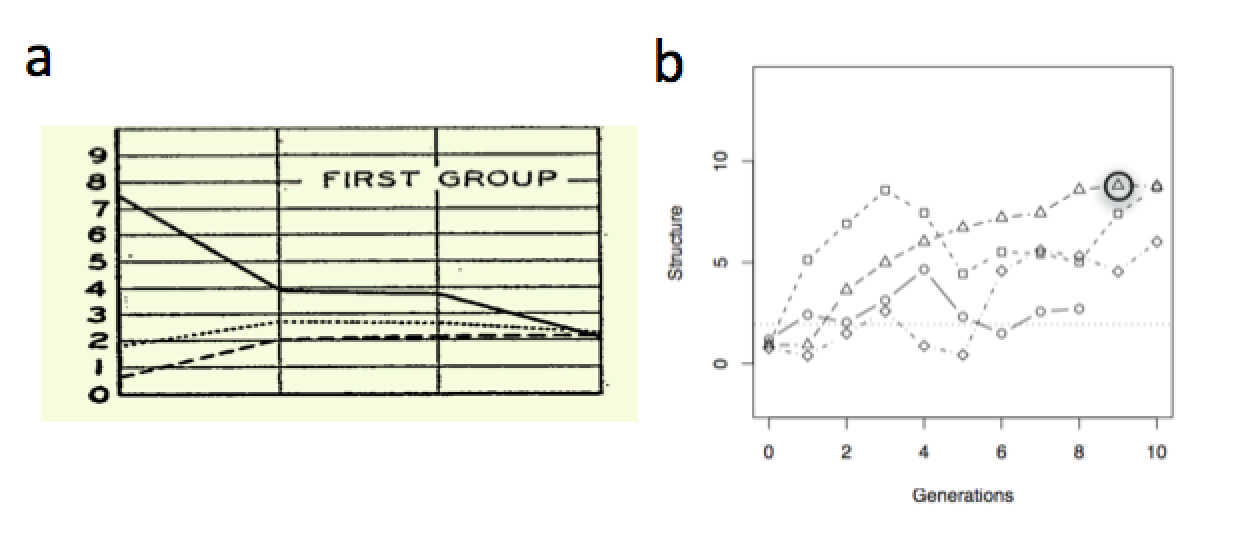
\includegraphics[width=5in]{figs/coordinatingmeaning.png}
\caption{\label{fig:results}  Plots reproduced from (a) Sherif (1935) and (b) Kirby,  Cornish, and Smith (2008). Plot (a) shows the median distance judgement (in inches) for three different subjects. The x-axis plots subjects performance on the task when completed individually, and then three subsequent periods in which the task was completed as a group (of 3 subjects).  Plot (b) shows the emergence of systematicity in the language across generations in the labeling task. Each line corresponds to a different set of people. Both plots suggest the emergence of systematicity, or conformity, within the group as a function of time. }
\end{center} 
\end{figure}

* unconcioncious, but increases with awareness

%%% Discourse and development %% 
\subsection{The relationship between discourse and developmental timscales} 
*cached equilibrium, generalization problem, learning to learn, overhypothes
\cite{smith2013learning}


%%% Development and language %% 
\subsection{The relationship between development and cultural timescales}
- christiasen and chater
\cite{smith2013learning}

Recent work using an artificial language paradigm tests this prediction. In a study by \citeA{kirby2008cumulative}, participants were presented with a novel language and asked to learn the pairings between words to novel images. For the first subject, the mappings between words and images was randomly generated. In the training phase, the subject was presented with an image and a label for that image. In the testing phase, they were shown a new image and asked to guess what word they thought was associated with that image. This first subject's responses were recorded, then divided into half (one half for training and one half for testing), and presented to a subsequent subject. This process repeated for a total of 10 subjects. Consistent with the Sherif (1935) results, it was predicted that language use would become more systematic over time. In particular, it was predicted that a pattern should emerge in the mapping between features of the stimuli (e.g.\ color, shape, etc.) and syllables in the novel words. This is exactly what was found (Figure 1b). As the number of generations increased, the language became more systematic. This pattern was observed across a four different ``strings" of participants.

It suggests that the conformity that takes place in the context of particular conversations (as demonstrated by Brennan and Clark, 1996) has larger consequences when aggregated across time and across a linguistic community. While conversations are the locus of conformity,  many small instances of conformity lead to highly regularized language patterns at the level of linguistic communities.


\subsection{Two case studies: Me and refComplex}

\subsection{Consequences for learning}
Christiansen and Chater
�	Frank - Inferring word meaning by assuming speakers are informative
\cite{smith2013learning}
�	Ali�s adjective paper
\cite{xu2007learning}

\subsection{An empirical challenge: Sufficient but not necessary mechanisms}
Parallels between development and language structure, and development and pragmatics in the moment of language use - ontological status of regularities just because they exist doesn't' mean we represent them. ontological status of these regularities -- difference between this and other laws of nature (e.g. physics) is that we can represent them -- general abstract rules (connect to symbol literature). The question is: do we represent these regularities explicitly?

\section{Conclusion}

\nocite{chater2010language}

\bibliographystyle{apacite}
\bibliography{biblibrary}

\end{document}

